
\documentclass[a4 paper,12pt]{article}
\usepackage[inner=2.0cm,outer=2.0cm,top=2.5cm,bottom=2.5cm]{geometry}
\usepackage{setspace}
\usepackage[rgb]{xcolor}
\usepackage{tabu}
\usepackage{multirow}
\usepackage{longtable}
\usepackage{graphicx}
\usepackage{verbatim}
\usepackage{longtable}
\usepackage{subcaption}
\usepackage{fancyhdr}
\usepackage[colorlinks=true, urlcolor=blue, linkcolor=blue, citecolor=blue]{hyperref}
\usepackage{booktabs}
\usepackage{amsmath,amsfonts,amsthm,amssymb}
\usepackage{setspace}
\usepackage{listings}
\usepackage{fancyhdr}
\usepackage{lastpage}
\usepackage{tikz}
\usetikzlibrary{positioning, arrows.meta}
\usepackage{extramarks}
\usepackage{ctex,amsmath,amsfonts,amssymb,bm,hyperref,graphicx}
%\lstset{
	%	commentstyle=\color{red!50!green!50!blue!50},%代码块背景色为浅灰色
	%	rulesepcolor= \color{gray}, %代码块边框颜色
	%	breaklines=true,  %代码过长则换行
	%	numbers=left, %行号在左侧显示
	%	numberstyle= \small,%行号字体
	%	keywordstyle= \color{blue},%关键字颜色
	%	frame=shadowbox,%用方框框住代码块
	%	basicstyle=\ttfamily
	%}
\definecolor{dkgreen}{rgb}{0,0.6,0}
\definecolor{mauve}{rgb}{0.9,0.1,0.4}
\definecolor{ash}{rgb}{0.8,0.8,0.8}
\lstset{ 
	language=Octave,                % the language of the code
	basicstyle=\ttfamily,           % the size of the fonts that are used for the code
	numbers=left,                   % where to put the line-numbers
	numberstyle=\small\color{gray},  % the style that is used for the line-numbers
	stepnumber=1,                   % the step between two line-numbers. If it's 1, each line
	% will be numbered
	numbersep=5pt,                  % how far the line-numbers are from the code
	backgroundcolor=\color{ash},      % choose the background color. You must add \usepackage{color}
	rulesepcolor= \color{gray}, %代码块边框颜色
	showspaces=false,               % show spaces adding particular underscores
	showstringspaces=false,         % underline spaces within strings
	showtabs=false,                 % show tabs within strings adding particular underscores
	frame=single,                   % adds a frame around the code
	rulecolor=\color{black},        % if not set, the frame-color may be changed on line-breaks within not-black text (e.g. commens (green here))
	tabsize=2,                      % sets default tabsize to 2 spaces
	captionpos=b,                   % sets the caption-position to bottom
	breaklines=true,                % sets automatic line breaking
	breakatwhitespace=false,        % sets if automatic breaks should only happen at whitespace
	title=\lstname,                   % show the filename of files included with \lstinputlisting;
	% also try caption instead of title
	frame=shadowbox,%用方框框住代码块
	keywordstyle=\color{blue},          % keyword style
	commentstyle=\color{dkgreen},       % comment style
	stringstyle=\color{mauve},         % string literal style
	escapeinside={\%*}{*)},            % if you want to add LaTeX within your code
	morekeywords={*,...}               % if you want to add more keywords to the set
}
\usepackage{chngpage}
\usepackage{soul,color}
\usepackage{graphicx,float,wrapfig}
\newcommand{\homework}[3]{
	\pagestyle{myheadings}
	\thispagestyle{plain}
	\newpage
	\setcounter{page}{1}
	\noindent
	\begin{center}
		\framebox{
			\vbox{\vspace{2mm}
				\hbox to 6.28in { {\bf Microeconomics \hfill} {\hfill {\rm #2} {\rm #3}} }
				\vspace{4mm}
				\hbox to 6.28in { {\Large \hfill #1  \hfill} }
				\vspace{3mm}}
		}
	\end{center}
	\vspace*{4mm}
}
\newcommand\numberthis{\addtocounter{equation}{1}\tag{\theequation}}
\renewcommand\contentsname{Contents}
\begin{document}
	\homework{Homework01}{Group45}{吴熙楠}
	\tableofcontents
	\newpage
\section{Problem\quad 1}
(a)This information will affect my decision to go to the concert. Because I like flank steak and I can eat in her party at no charge. So going to the concert is the opportunity cost if I think the value of eating the flank steak is greater than the value of going to the concert. The opportunity cost of going to the concert becomes larger than before, but the opportunity cost of going to the party has nnot changed. So it will affect my decision.
\par (b)This information will not affect my decision to go to the concert. Although I know that the price of the ticket is \$10 and the ticket is non-refundable. And it is the sunk cost, so it should not affect my decision after I buy it. Going to the concert is the opportunity cost if I go to the party, but I politely deciline because I really want to go to the concert. The opportunity cost has not changed, so I don't change my decision. 
\section{Problem\quad 2}
(a)As shown in the table above, 0 hour of study time corresponds to 0 point, 1 hour corresponds to 10 points, 2 hours correspond to 13 points, 3 hours correspond to 12 points, 4 hours correspond to 5 points. So we can see that 2 hours of study time will make me get a maximum of 13 points. That is to say, if I study in an optimal way, I can earn 13 points. 
\par (b)We know that when our marginal benefits are larger than our marginal cost, our total points will increase. So If we need to find the optimal number of hours for which we should study, we can compare marginal benefits with marginal cost. Actually the total points are largest when the marginal benefits are equal to the marginal cost, but because the data points are discrete, we cannot achieve strict equality. Then we find that when the study time is 2 hours, the marginal benefits are larger than the marginal cost, but when the study time is 3 hours, the marginal benefits are smaller than the marginal cost. So 2 is the optimal number of hours for which we should study.
\section{Problem\quad 3}
\newpage
(a)	\begin{figure}[H]
	\centering
	\hspace{2em}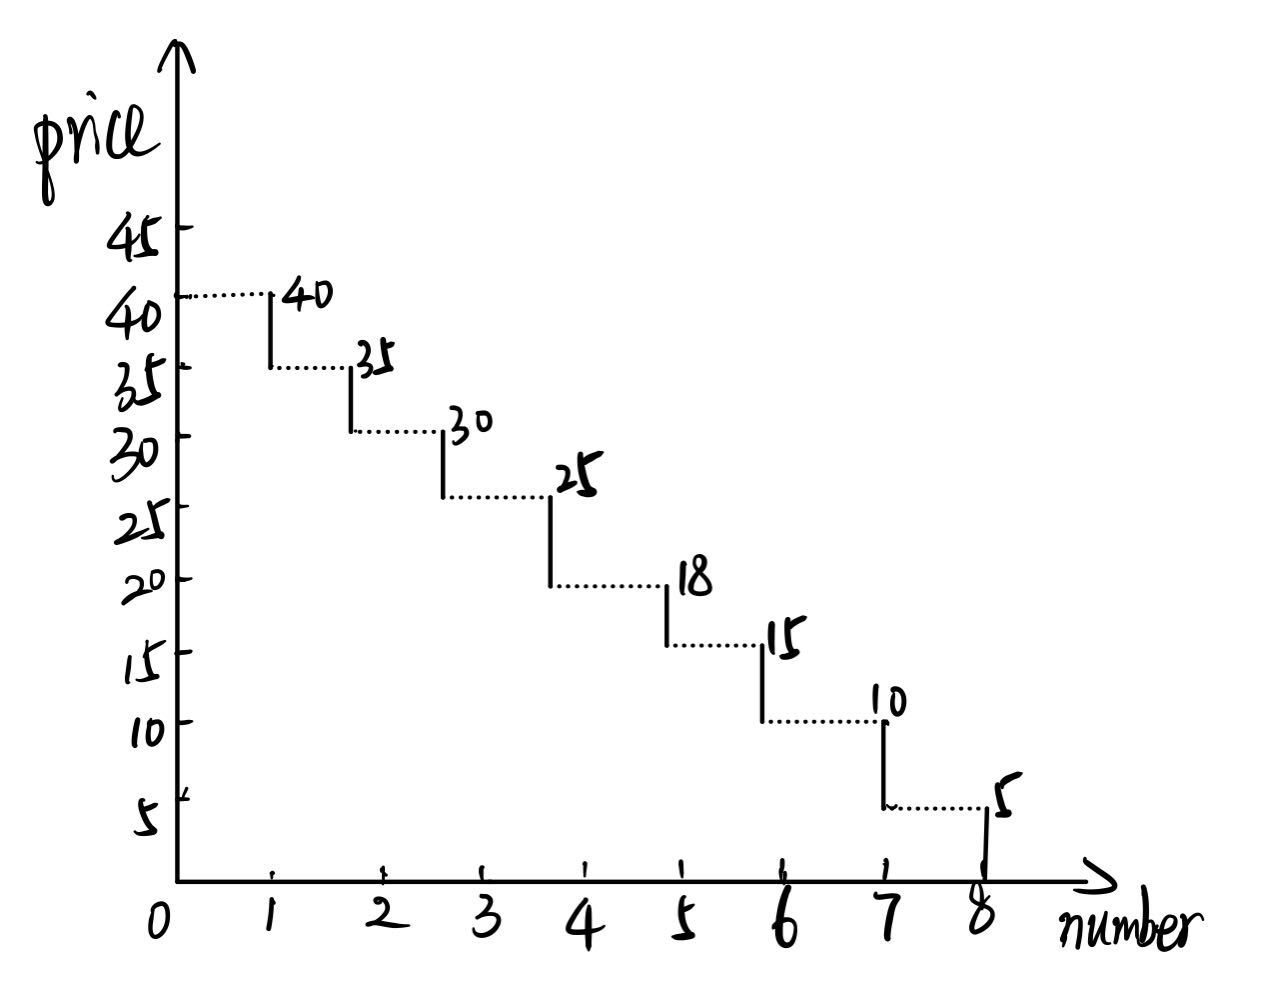
\includegraphics[width=0.3\linewidth]{pic/curve.jpg}
	\caption*{\tiny The Market Demand Curve
	}
\end{figure}
\par (b)\begin{figure}[H]
	\centering
	\hspace{2em}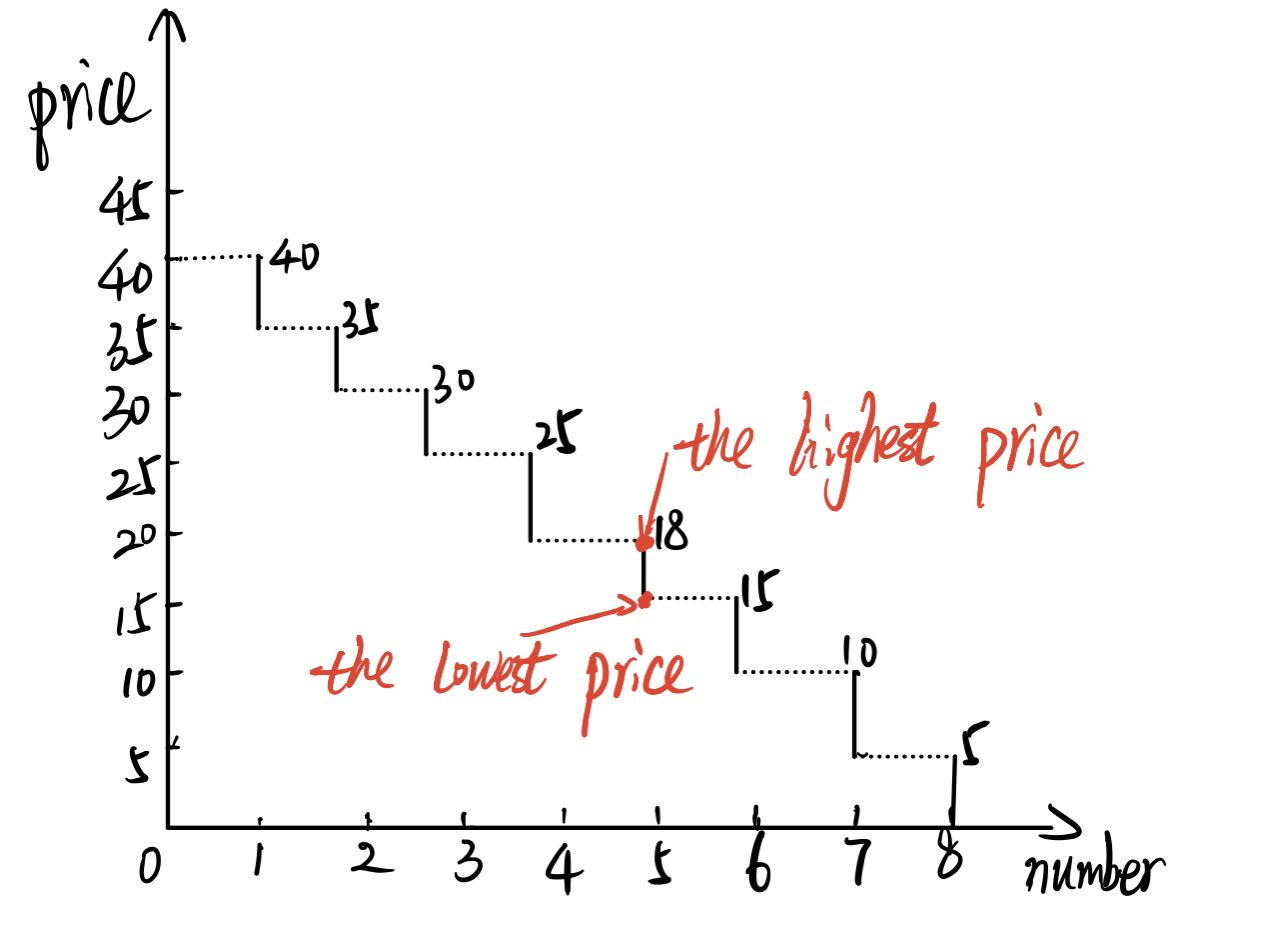
\includegraphics[width=0.3\linewidth]{pic/curve-hl.jpg}
	\caption*{\tiny The Market Demand Curve
	}
\end{figure}
\par According to the figure above, the highest price that would make the demand of apartments equal to 5 units is 18.
\par (c)\begin{figure}[H]
	\centering
	\hspace{2em}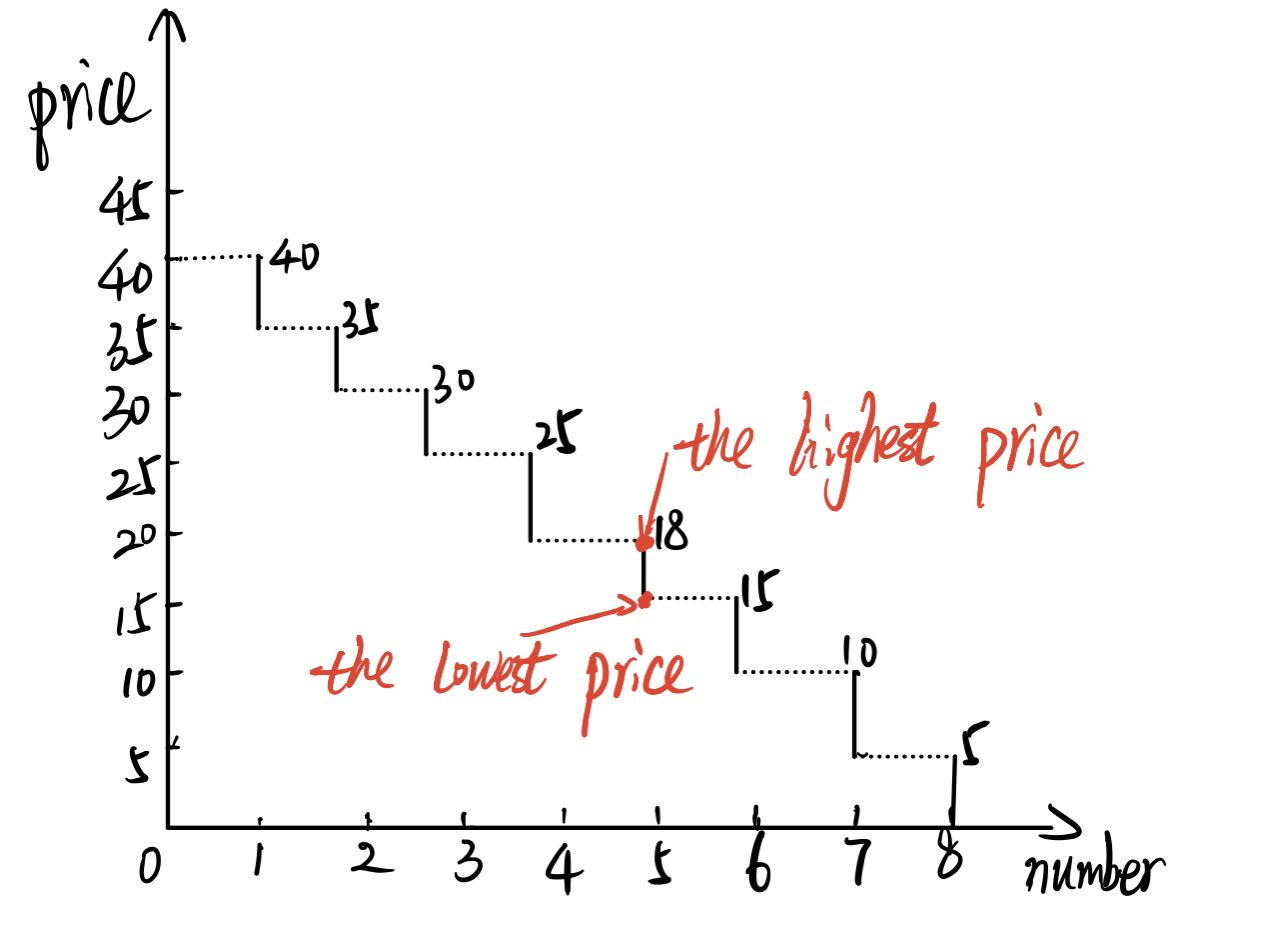
\includegraphics[width=0.3\linewidth]{pic/curve-hl.jpg}
	\caption*{\tiny The Market Demand Curve
	}
\end{figure}
\par According to the figure above, the highest price that would make the demand of apartments equal to 5 units is 15.
\par (d)Because the supply of four apartments is less than the demand, the person with higher reservation price will get the apartment. In this case, A,C,D,G will get the apartments.
\par (e)If the supply of apartments increases to 6 units, the range of equilibrium prices will go down because of the rising supply. The range of equilibrium prices will be $10\sim 15$.
\section{Problem\quad 4}
(a)\begin{table}[H]
	\centering
	\caption*{Price Revenue Statement}
	\begin{tabular}{c|*{8}{c}}
		\toprule[0.5mm]
		Number&1&2&3&4&5&6&7&8\\
		\midrule
		Price&40&35&30&25&18&15&10&5\\
		Revenue&40&70&90&100&90&90&70&40\\
		\bottomrule[0.5mm]
	\end{tabular}
\end{table}
\par (b)From the table above, renting out four apartments yields the most. So in this case, A,C,D,G will get the apartments.
\par (c)In this case, the top 5 prices are 40,35,30,25,18. So he can earn 148 if he rents all 5 apartments.
\par (d)In the same way, A,C,D,G,E will get the 5 apartments.
\par (e)In the case of (d), the landlord can earn more and there are also more apartments available to rent to others. So the outcome in (d) is Pareto efficient, and the market outcome is Pareto inefficient.
\section{Problem\quad 5}
(a)1.If we assume that the tax rate is $\tau$ and the previous reservation price is $a$. Then his reservation price will become $a(1-\tau)$. So in this case, if there are 5 apartments to be rented,  the maximum equilibrium price is $18(1-\tau)$.\quad2.If we assume that the tax is $r$ and the previous reservation price is $a$. Then his reservation price will become $a-r$ (of course $r\leq a$). So in this case, if there are 5 apartments to be rented,  the maximum equilibrium price is $18-r$.
\par (b)Whether we use the tax rate or the tax to calculate, the result is allways the same compare to what happens if the tax is imposed on the landlord. The landlord's
profit is allways $a(1-\tau)$ or $a-r$, and the renters allways cost $a$ for renting the apartments.
\end{document} 
